\subsection{Indflydelse af basrefleks}
Højtalerkabinettet har et hul på forsiden, på siden og et på bagsiden hvori det er muligt, at installere basreflekser i forskellige længder - dog kun en basrefleks ad gangen. I første omgang er der kun blevet set på hvordan basreflekser af forskellige længder påvirker membranens karakteristik, når basrefleksen er placeret foran på højtaleren. Resultatet af disse målinger i vist på den nedenstående figur:
\begin{figure}[H]
	\centering
	\vspace{-12pt}
	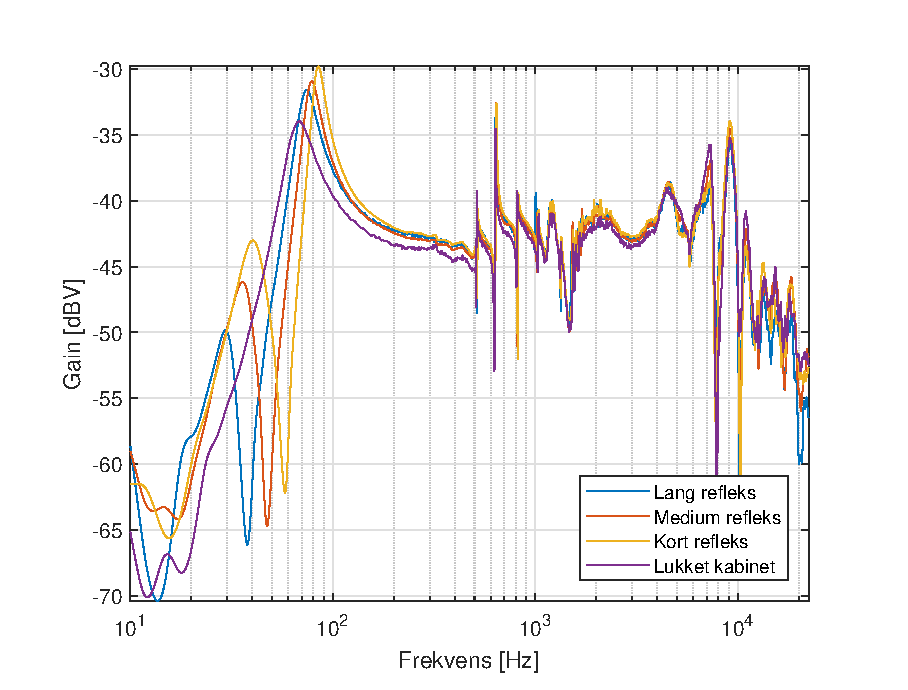
\includegraphics[width=\textwidth]{Pics/BassReflexMembrane}
	\caption{Indflydelse af forskellige længder basrefleks}
\end{figure}

På figuren ses også frekvenskarakteristikken for et lukket kabinet - altså et kabinet uden basrefleks. Det ses, at det lukkede kabinets frekvenskarakteristik er meget lav ved de lave frekvenser. Det ses også, at der tilføjes et forstærkningspeak når der tilføjes en basrefleks. Placeringen af denne peak afhænger af refleksens længde. Jo længere røret er, jo længere nede i frekvensspektret kommer peaken til at ligge. Omvendt vil en længere basrefleks også betyde, at peaken bliver mindre - altså mindre forstærkning.
\begin{table}[H]
	\centering
	\begin{tabular}{l|c|c|c|c}
		& Lukket kabinet & Lang refleks & Medium refleks & Kort refleks \\ \hline
		Dyk fra enhed {[}Hz{]}    & -              & 38              & 47                & 58             \\
		Dyk fra enhed {[}dB{]}    & -              & -66             & -65               & -62            \\
		Peakfrekvens {[}Hz{]}     & 68             & 74              & 78                & 85             \\
		Peakforstærkning {[}dB{]} & -34            & -32             & -31               & -30           
	\end{tabular}
	\caption{Måleresultater}
\end{table}

Ud fra den ovenstående figur ses det også, at basrefleksen ikke vil påvirke membranens frekvenskarakteristik ved frekvenser over \SI{500}{\hertz}.